\documentclass{../khlslides}


\title[Fundamenten]{Conditionals}
\author{Fr\'ed\'eric Vogels}


\pgfkeys{/tikz/flowchart/node/.style={rectangle,fill=blue,opacity=0.5,text opacity=1,drop shadow,inner sep=2mm}}
\pgfkeys{/tikz/flowchart/arrow/.style={-latex,flowchart/arrowline}}
\pgfkeys{/tikz/flowchart/arrowline/.style={thick}}


\newcommand{\lcurly}{{\tt{\char '173}}}
\newcommand{\link}[2]{\href{#1}{\beamergotobutton{#2}}}
\newcommand{\PLACEHOLDER}[1]{\ensuremath{\langle}\textrm{\textit{#1}\ensuremath{\rangle}}}



\begin{document}

\begin{frame}
  \titlepage
\end{frame}

\begin{frame}
  \frametitle{Basiselementen Algoritmes}
  \begin{center}
    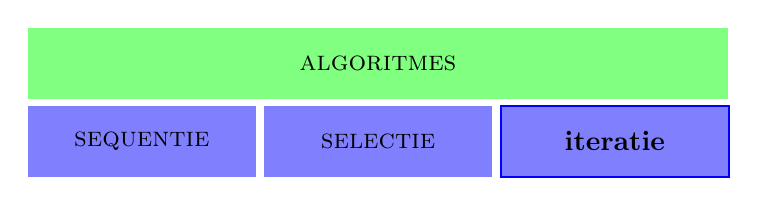
\begin{tikzpicture}[building block/.style={minimum width=2.9cm,minimum height=.9cm,fill=blue!50,font=\sc},
                        algorithm/.style={minimum width=8.9cm,minimum height=.9cm,fill=green!50,font=\sc}]
      \node[building block,anchor=south west] at (0,0) { sequentie };
      \node[building block,anchor=south west] at (3,0) { selectie };
      \node[building block,anchor=south west,draw=blue,thick] at (6,0) { \bfseries iteratie };
      \node[algorithm,anchor=south west] at (0,1) { algoritmes };
    \end{tikzpicture}
  \end{center}
\end{frame}

\begin{frame}
  \frametitle{Rad van Fortuin}
  \begin{center}
    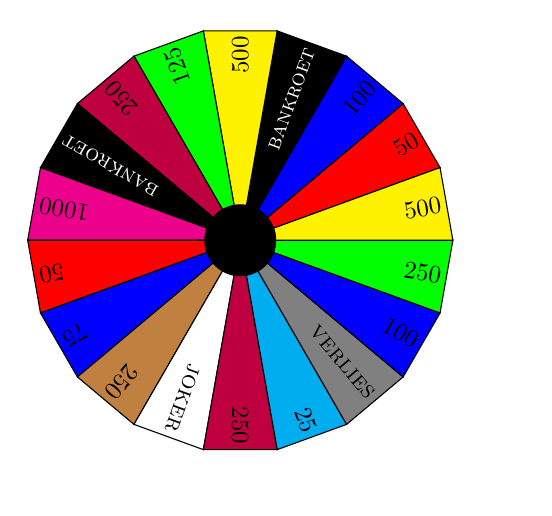
\begin{tikzpicture}[scale=.9,transform shape]
      \path[use as bounding box] (-3,-3.5) rectangle (4,3);

      \foreach[count=\i] \text/\c in {50/red,100/blue,{\color{white}\sc\small bankroet}/black,500/yellow,125/green,250/purple,{\color{white}\sc\small bankroet}/black,1000/magenta,50/red,75/blue,250/brown,{\sc joker}/white,250/purple,25/cyan,{\sc verlies}/gray,100/blue,250/green,500/yellow} {
        \pgfmathparse{20}\let\deltaangle\pgfmathresult
        \pgfmathparse{\i * \deltaangle}\let\startangle\pgfmathresult
        \pgfmathparse{\startangle + \deltaangle/2}\let\midangle\pgfmathresult
        \pgfmathparse{\startangle + \deltaangle}\let\endangle\pgfmathresult
        \draw[fill=\c] (0,0) -- (\startangle:3cm) -- (\endangle:3cm) -- cycle;
        \coordinate (cell \i) at (\midangle:3cm);
        \node[anchor=east,rotate=\midangle] at (\midangle:3cm) {\text};
      }
      \draw[fill=black] (0,0) circle (.5cm);
    \end{tikzpicture}
    \vskip4mm
    We herbezoeken hetzelfde voorbeeld
  \end{center}
\end{frame}

{
\pgfkeys{
  /wof/sequence point/.cd,
  placement/.initial=above,
  /wof/sequence link/.cd,
  label/.initial={}
}
\newcommand{\seqpoint}[3][]{{
  \pgfkeys{/wof/sequence point/.cd,#1}
  \pgfkeys{/wof/sequence point/placement/.get=\placement}
  \draw[sequence point] (#2) circle (.05)
                        node[sequence point label,\placement] {#3};
}}
\newcommand{\seqlink}[3][]{{
  \pgfkeys{/wof/sequence link/.cd,#1}
  \pgfkeys{/wof/sequence link/label/.get=\seqlinklabel}
  \draw[sequence link] (#2) -- (#3) node[midway,sloped,yshift=1mm,font=\tiny,black] {\seqlinklabel};
}}

\newcommand{\singleround}{
        \coordinate (init) at (0,0);
        \coordinate (turn wheel) at ($ (init) + (1,2) $);
        \coordinate (bankruptcy lose money) at ($ (turn wheel) + (1,1.5) $);
        \coordinate (bankruptcy next player) at ($ (bankruptcy lose money) + (2,0) $);
        \coordinate (pass) at ($ (turn wheel) + (3,0.5) $);
        \coordinate (joker) at ($ (turn wheel) + (3,-0.5) $);
        \coordinate (consonant) at ($ (turn wheel) + (1,-1.5) $);
        \coordinate (show consonant) at ($ (consonant) + (2,0) $);
        \coordinate (no consonants) at ($ (show consonant) + (1,-0.5) $);
        \coordinate (end consonants) at ($ (show consonant) + (2,0) $);
        \coordinate (exit) at ($ (init) + (8,0) $);
        \coordinate (vowel) at ($ (init) + (1,-2) $);
        \coordinate (buy vowel) at ($ (vowel) + (1.5,0) $);
        \coordinate (show vowels) at ($ (buy vowel) + (1.5,0) $);
        \coordinate (no vowels) at ($ (show vowels) + (1.5,.5) $);
        \coordinate (end vowels) at ($ (show vowels) + (3,0) $);

        \seqlink[label=rad]{init}{turn wheel}
        \seqlink[label=bankroet]{turn wheel}{bankruptcy lose money}
        \seqlink{bankruptcy lose money}{bankruptcy next player}
        \seqlink[label=verlies beurt]{turn wheel}{pass}
        \seqlink[label=joker]{turn wheel}{joker}
        \seqlink[label=else]{turn wheel}{consonant}
        \seqlink{consonant}{show consonant}
        \seqlink[label=0]{show consonant}{no consonants}
        \seqlink[label=1+]{show consonant}{end consonants}
        \seqlink{no consonants}{end consonants}
        \seqlink{end consonants}{exit}
        \seqlink{joker}{exit}
        \seqlink{pass}{exit}
        \seqlink{bankruptcy next player}{exit}
        \seqlink[label=klinker]{init}{vowel}
        \seqlink{vowel}{buy vowel}
        \seqlink{buy vowel}{show vowels}
        \seqlink[label=0]{show vowels}{no vowels}
        \seqlink{no vowels}{end vowels}
        \seqlink[label=1+]{show vowels}{end vowels}
        \seqlink{end vowels}{exit}

        \seqpoint[placement=left]{init}{rad/klinker}
        \seqpoint[placement=left]{turn wheel}{draai rad}
        \seqpoint{bankruptcy lose money}{score = 0}
        \seqpoint{bankruptcy next player}{huidigeSpeler++}
        \seqpoint{pass}{huidigeSpeler++}
        \seqpoint{joker}{jokers++}
        \seqpoint[placement=below]{consonant}{gok medeklinker}
        \seqpoint{show consonant}{toon}
        \seqpoint[placement=below]{no consonants}{huidigeSpeler++}
        \seqpoint{end consonants}{}
        \seqpoint[placement=below]{vowel}{gok klinker}
        \seqpoint[placement=below]{buy vowel}{score -= 50}
        \seqpoint{show vowels}{toon}
        \seqpoint{no vowels}{huidigeSpeler++}
        \seqpoint{end vowels}{}
        \seqpoint{exit}{}
}

\begin{frame}
  \frametitle{Rad van Fortuin: E\'en Ronde}
  \begin{center}
    \begin{tikzpicture}[sequence point/.style={blue!50,thick,fill=white},
                        sequence point label/.style={font=\tiny,black},
                        sequence link/.style={blue!50,thick}]
      \singleround
    \end{tikzpicture}
  \end{center}
\end{frame}

\begin{frame}
  \frametitle{Rad van Fortuin: E\'en Ronde}
  \begin{center}
    \begin{tikzpicture}[sequence point/.style={blue!50,thick,fill=white},
                        sequence point label/.style={font=\tiny,black},
                        sequence link/.style={blue!50,thick}]
      \begin{scope}[scale=0.25,transform shape]
        \singleround
      \end{scope}

      \begin{scope}[scale=0.25,transform shape,xshift=10cm]
        \singleround
      \end{scope}
    \end{tikzpicture}
  \end{center}
\end{frame}
}

\end{document}

%%% Local Variables: 
%%% mode: latex
%%% TeX-master: t
%%% End: 
